\documentclass[aspectratio=169]{beamer}
\usetheme{Madrid}
\usecolortheme{default}

\usepackage[T1]{fontenc}
\usepackage{lmodern}
\usepackage{graphicx}
\usepackage{tikz}
\usepackage{pgfplots}
\pgfplotsset{compat=1.14}
\usepackage{anyfontsize}
\usepackage{xspace}
\usepackage{amsmath}
\usepackage{booktabs}
\usepackage{caption}
\usepackage{algpseudocode}
\usepackage{hyperref}
\usepackage{graphicx}
\newcommand{\cev}[1]{\reflectbox{\ensuremath{\vec{\reflectbox{\ensuremath{#1}}}}}}


\title[Week 1]
{Variational Canonical Correlation Analysis}

\subtitle{Week 1}

\author[] % (optional, for multiple authors)
{
Konstantin Yakovlev \inst{1} \and
}

\institute[] % (optional)
{
  \inst{1}%
  MIPT \\
  Moscow, Russia
}

\date[MIPT 2023] % (optional)
{MIPT 2023}

% \logo{\includegraphics[height=0.8cm]{logo_uoft}}

\definecolor{uoftblue}{RGB}{6,41,88}
\setbeamercolor{titlelike}{bg=uoftblue}
\setbeamerfont{title}{series=\bfseries}

\begin{document}

\frame{\titlepage}

\begin{frame}{Deep Variational Canonical Correlation Analysis\footnote{\href{https://arxiv.org/pdf/1610.03454.pdf}{Wang W. et. al, Deep Variational Canonical Correlation Analysis, 2017}}}
    \textbf{Challenge}: it is hard to satisfy the constraints set by Deep Canonical \\
    \textbf{Solution}: extends the latent variable interpretation to nonlinear observation models.
    \begin{minipage}{0.33\textwidth}
        \textbf{DCCA}:
        \begin{small}
        \begin{align*}
            \max_{f, g, U, V}\mathrm{tr}(U^\top f(X)g(Y)^\top V) \\
            \mathrm{s.t.} \quad U^\top(f(X)f(X)^\top)U = \\
            V^\top(g(Y)g(Y)^\top)V = N\cdot I.
        \end{align*}
        \end{small}
    \end{minipage}\hfill
    \begin{minipage}{0.33\textwidth}
        \textbf{Probalistic CCA vs VCCA}: \\
        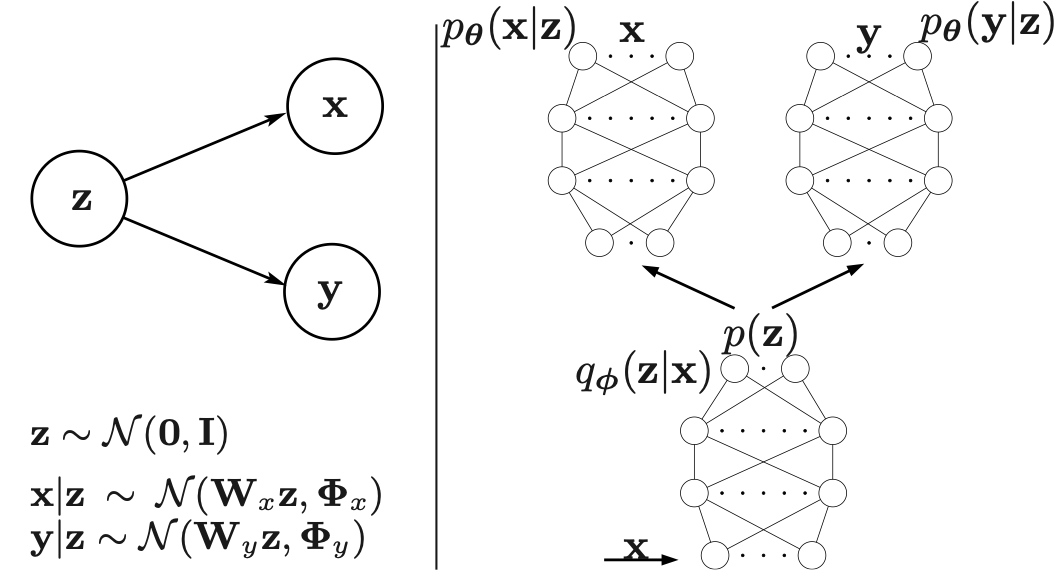
\includegraphics[width=\textwidth]{figures/fig1.png}
    \end{minipage}\hfill
    \begin{minipage}{0.33\textwidth}
        \textbf{VCCA-private}:  the challenge is that large variations in the input space can not be explained by $\mathbf{z}$.\\
        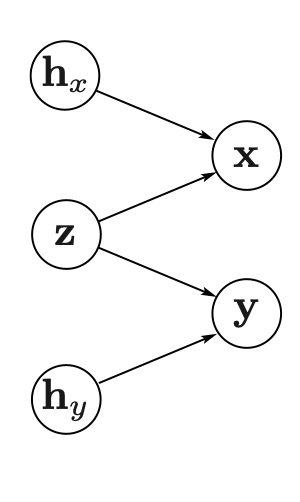
\includegraphics[width=0.4\textwidth]{figures/fig2.png}
    \end{minipage}
    \textbf{Results}: outstanding performance with reduced training efforts.
    
\end{frame}


\begin{frame}{Variational Interpretable Deep Canonical Correlation Analysis\footnote{\href{https://openreview.net/pdf?id=Gzare7_sTAJ}{Qui L. et. al, Variational Interpretable Deep Canonical Correlation Analysis, 2022}}}
    \textbf{Challenge}: it is challenging to build an interpretable model understanding. \\
    \textbf{Solution}: interpretable sparsity prior.\\
    \begin{minipage}{0.33\textwidth}
        \textbf{Sparsity prior}
        \begin{small}
        \begin{align*}
            &Z \sim N(0, I), \; Z^m \sim N(0, I), \\
            &X^m \sim N(f_m(\Lambda^m Z + W^mZ^m), \Psi^m) \\
            &\gamma^2_{mj} \sim \Gamma((d_m + 1)/2, \lambda^2 / 2) \\
            &\Lambda^{(m)}_{., j}, W^{(m)}_{., j} \sim N(0, \gamma^2_{mj}I)
        \end{align*}
        \end{small}
    \end{minipage}\hfill
    \begin{minipage}{0.33\textwidth}
        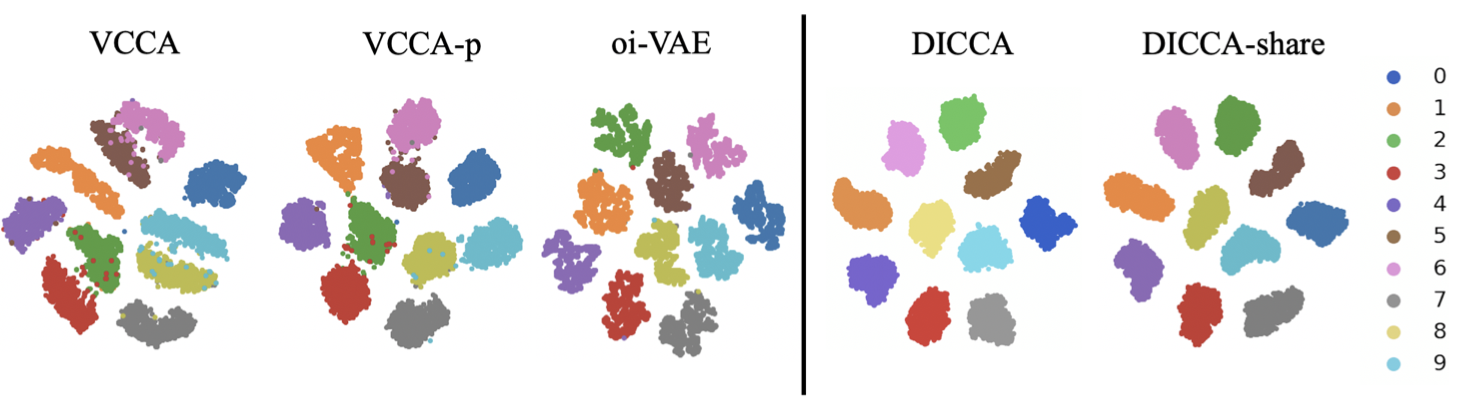
\includegraphics[width=1.0\textwidth]{figures/fig3.png}
        The learned features of the images are well separated.
    \end{minipage} \hfill
    \begin{minipage}{0.33\textwidth}
        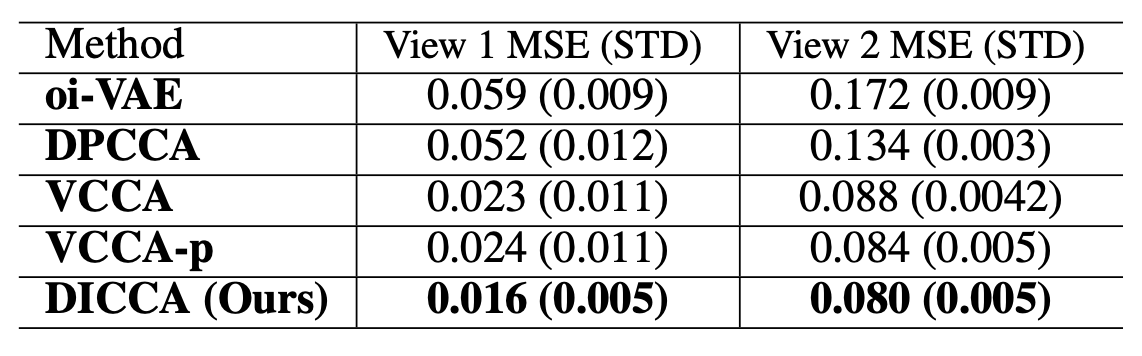
\includegraphics[width=\textwidth]{figures/fig4.png}
        The proposed method outperforms all existing baselines.
    \end{minipage}
\end{frame}




\end{document}